\documentclass[tikz,border=8pt]{standalone}
\usepackage[T1]{fontenc}
\usepackage{tikz}
\usetikzlibrary{arrows.meta,positioning,fit}
\definecolor{blue}{RGB}{32,94,180}
\definecolor{green}{RGB}{49,142,109}
\definecolor{purple}{RGB}{112,94,174}
\definecolor{gold}{RGB}{190,132,45}
\definecolor{textgray}{RGB}{38,45,56}
\tikzset{
  box/.style={draw=#1, fill=#1!8, rounded corners=3pt, thick, align=center,
    minimum width=31mm, minimum height=10mm, text=textgray, font=\sffamily\small},
  wide/.style={draw=#1, fill=#1!8, rounded corners=3pt, thick, align=center,
    minimum width=50mm, minimum height=11mm, text=textgray, font=\sffamily\small},
  arrow/.style={-{Latex[length=2.2mm]}, thick, draw=textgray!70}
}
\begin{document}
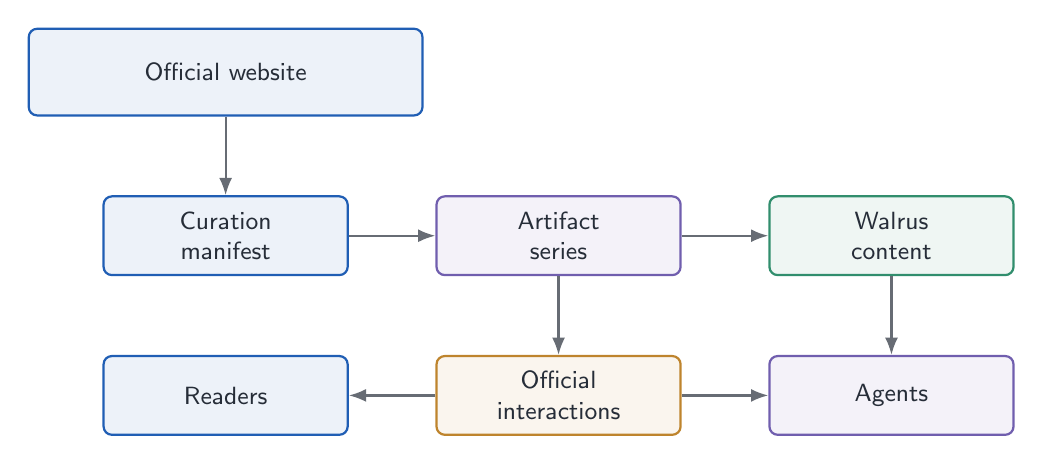
\begin{tikzpicture}[node distance=10mm and 11mm]
  \node[wide=blue] (site) {Official website};
  \node[box=blue, below=of site] (manifest) {Curation\\manifest};
  \node[box=purple, right=of manifest] (series) {Artifact\\series};
  \node[box=green, right=of series] (package) {Walrus\\content};
  \node[box=gold, below=of series] (interactions) {Official\\interactions};
  \node[box=blue, below=of manifest] (readers) {Readers};
  \node[box=purple, below=of package] (agents) {Agents};
  \draw[arrow] (site) -- (manifest);
  \draw[arrow] (manifest) -- (series);
  \draw[arrow] (series) -- (package);
  \draw[arrow] (series) -- (interactions);
  \draw[arrow] (package) -- (agents);
  \draw[arrow] (interactions) -- (readers);
  \draw[arrow] (interactions) -- (agents);
\end{tikzpicture}
\end{document}
